\section{Руководство пользователя}

\subsection{ Особенности реализации PIC в программе \prognv }

\textbf{Расчетная область и источники частиц.}
Перед началом моделирования нужно определить расчетную область и заселить ее частицами.
Epifc-v0.01 поддерживает расчетную область только прямоугольной формы. 
Что касается генерации частиц - то пока есть возможность задать только один источник.
Кроме того, генерация новых частиц во время работы тоже пока не поддерживается.
\todo{При дискретизации области используется прямоугольная сетка с фиксированным шагом.}
\begin{figure}[h]
  \centering
  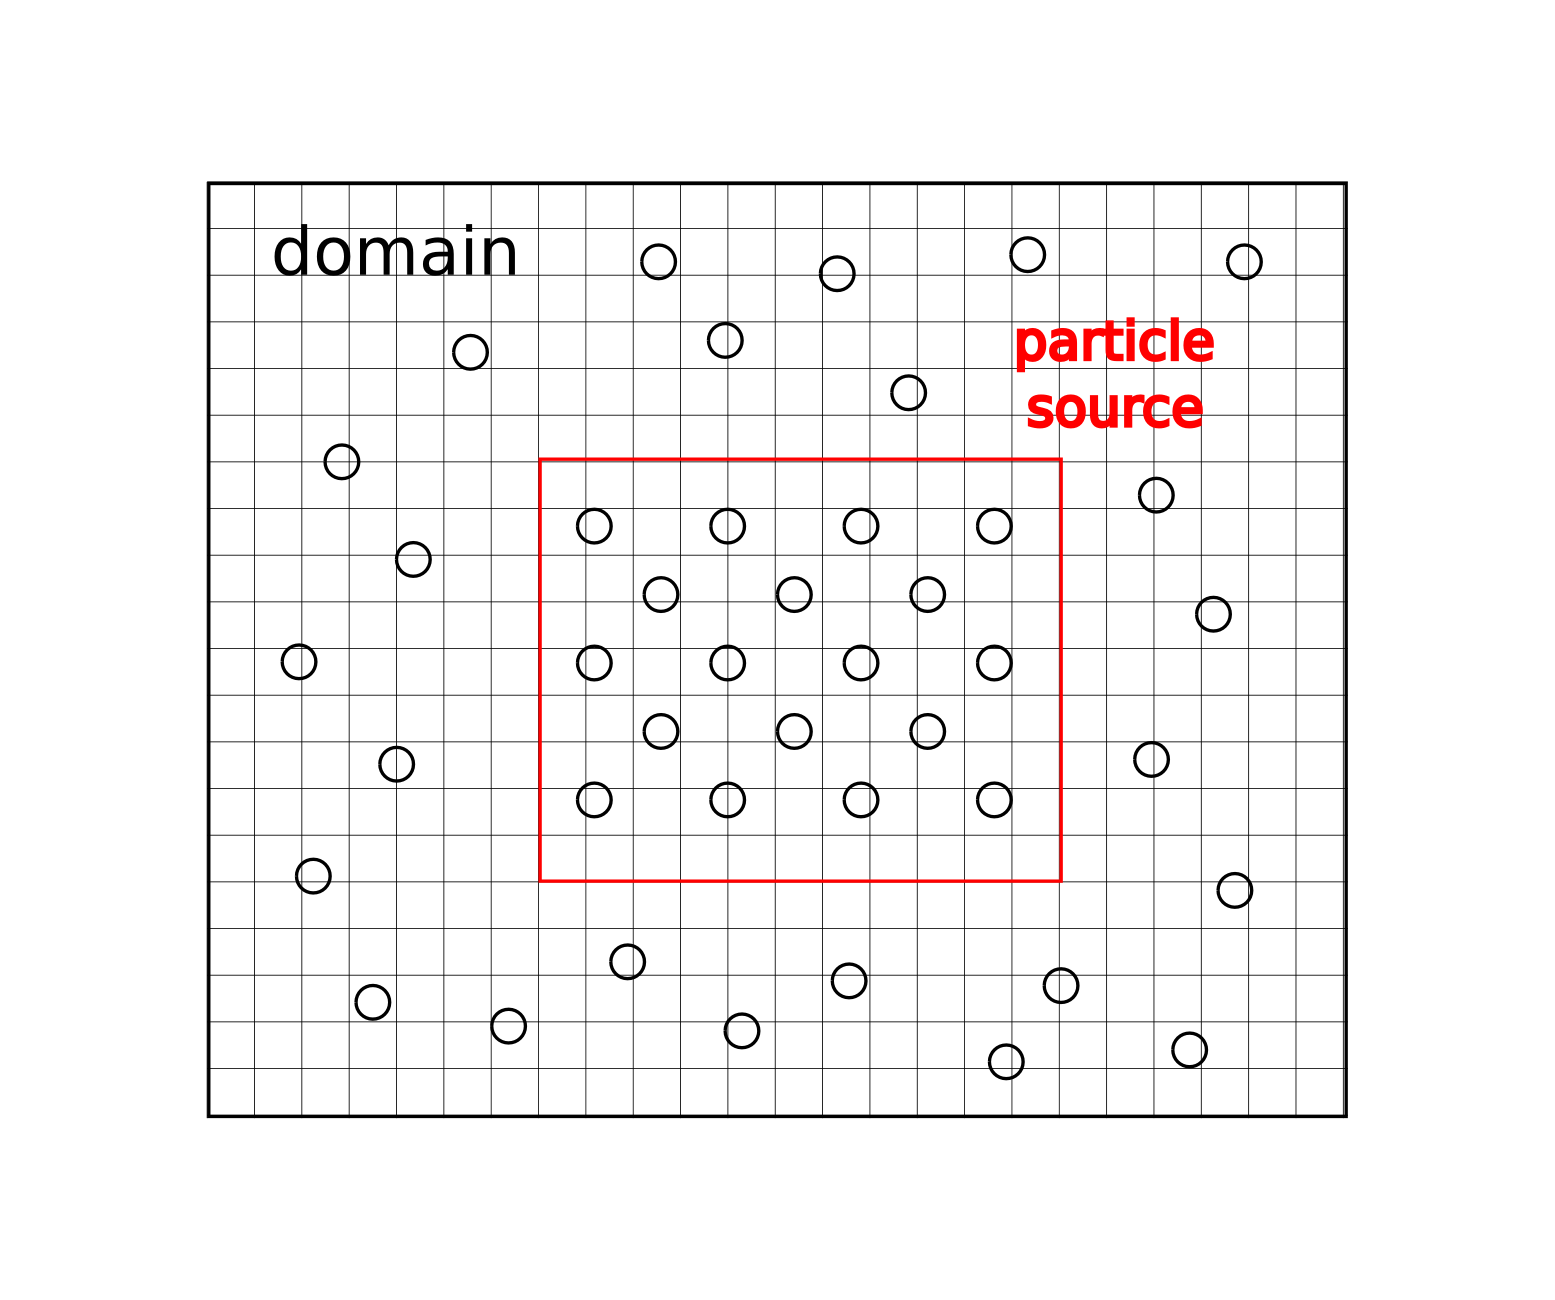
\includegraphics[scale=0.8]{./figs/domain.png}
  \caption{
    Схематичное изображение расчетной области программы.
    \todo{надо его как-то по-аккуратнее сделать}
  }
\end{figure}



\textbf{Связь характеристик макрочастиц с концентрацией реальных частиц и плотностью заряда в области.}
У каждой макрочастицы есть заряд и масса. 
Если концентрация реальных частиц
массой $m_{real}$ и зарядом $q_{real}$
в объеме $V$ равна $n_0\, [1/cm^2]$, 
то масса $m$ и заряд $q$ каждой макрочастицы определяются соотношениями
\begin{gather}
  m = m_{real} \frac{ n_0 V }{ N },
  \quad
  q = q_{real} \frac{ n_0 V }{ N },
\end{gather}
где $N$ - число макрочастиц.
Пользователю необходимо задать массу $m$, заряд $q$ и число макрочастиц $N$
для каждого источника ( см. \ref{sec:config_file} ).

\textbf{Распределение скоростей и координат генерируемых частиц.}
По координатам - равномерно в прямоугольнике.
По импульсам - максвелловское распределение.
\begin{gather}
  f( \vec{p} ) dp = \frac{1}{ 2 \pi m \theta } e^{ - \dfrac{ p_x^2 + p_y^2 }{ 2 m \theta } }
\end{gather}
где $\theta = k T$, $k$ - постоянная Больцмана, $T$ - температура.
В конфигурационном фаиле необходимо задать $\theta$ для каждого источника.


После инициализации частиц запускается алгоритм PIC. 
Вначале происходит интерполяция зарядов макрочастиц на узлы сетки.
Предполагается, что частицы вносят вклад только в ближайшие узлы. 
\todo{Форма частиц - ступенька ( поискать официальное название для этого ).}
\todo{Вставить картинку.}

\todo{Здесь оставить только общие уравнения. Дискретные убрать в раздел с описанием программы.}

Следующий шаг - расчет потенциалов. 
Epicf-v0.01 не поддерживает магнитное поле
и использует только электрическое ( электростатическая модель, ES-PIC ).
Для его нахождения нужно решить уравнение Пуассона:
\begin{gather}
  \Delta \phi = - 4 \pi \rho
\end{gather}
Поддерживаются граничные условия только 1 рода ( на потенциал, а не на поле ).
Они задаются в конфигурационном фаиле.

По найденным значениям потенциала расчитывается значение поля в узлах решетки:
\begin{gather}
  \vec{ E } = - \nabla \phi
\end{gather}

Затем обновляются импульсы и координаты частиц
( при этом происходит обратная интерполяция полей из узлов решетки на частицы ).
\begin{gather}
  \frac{ d \vec{p} }{ d t } = \vec{ F } = q \vec{ E }
  \\
  \frac{ d \vec{r} }{ d t } = \frac{ \vec{p} }{ m }
\end{gather}
Используется схема Leap-frog ( см. след раздел ).
\todo{ дописать пару слов про нее.  }

\textbf{Запись в фаил.}
В конце временного шага можно сохранить результаты расчетов в фаил. 
Записывается вся информация, необходимая для возобновления расчетов.
Детально формат фаила описан в \todo{следующем} разделе. 
Имя выходного фаила генерируется по параметрам в конфигурационном фаиле.
Номер временного шага для записи тоже берется из конфига.




\subsection{ Параметры конфигурационного фаила }
\label{sec:config_file}

Для пользователя взаимодействие с программой должно ограничиваться изменениями в конфигурационном фаиле.

Пример конфигурационного фаила идет в комплекте с программой.
\begin{verbatim}
# PIC simulation config.
# Do not change section and field names.

[Time grid]
total_time = 1.0
time_step_size = 0.1

[Spatial mesh]
grid_x_size = 15.0
grid_x_step = 0.3
grid_y_size = 10.0
grid_y_step = 0.1

[Test particle source]
particle_source_number_of_particles = 300
particle_source_x_left = 1.0
particle_source_x_right = 10.0
particle_source_y_bottom = 1.0
particle_source_y_top = 8.0
particle_source_temperature = 10.0
particle_source_charge = 1.0
particle_source_mass = 1.0

[Boundary conditions]
boundary_phi_left = 100.0
boundary_phi_right = 300.0
boundary_phi_bottom = 400.0
boundary_phi_top = 200.0

[Output filename]
# No quotes; no spaces till end of line
output_filename_prefix = out/out_new
output_filename_suffix = .dat
\end{verbatim}
Смысл большей части полей должен быть ясен из названия.
Названия секций и имена полей менять нельзя. 
Порядок менять можно.

Epicf ничего не знает о размерностях, поэтому задание параметров с согласованными единицами измерения - задача пользователя.
\todo{Единицы измерения лучше выбирать так, чтобы все параметры получались близкими к единице, т.е. чтобы не возникало
очень маленьких или очень больших чисел - насколько это реализуемо? Наверное лучше задать границы области очень большими
числами, а параметры частиц сделать близкими к единице.}

Тестовый конфиг соответствует следующей ситуации. Все меряется в СГС.
Есть область 15x10 см ( \texttt{grid\_x\_size, grid\_y\_size} ), внутри нее есть источник частиц размером 9 x 7 см 
( \texttt{particle\_source\_x\_left, ..., particle\_source\_y\_top}; см. также рис ? ).
В начальный момент времени в этом источнике находится 300 макрочастиц ( \texttt{particle\_source\_number\_of\_particles} ).
На границах области поддерживается некая разность потенциалов 
( \texttt{ boundary\_phi\_left, ..., boundary\_phi\_top }; единицы измерения потенциала - см. ниже ). 
Нужно смоделировать 1 сек. ( \texttt{total\_time} ) эволюции этой системы.

Допустим, что источник излучает ионы аргона Ar$^{+}$. 
Реальная масса и заряд одного иона 
\begin{gather}
  m_{real}  
  = \dfrac{ \mu }{N_A} 
  = \dfrac{40 \mbox{[г/моль]} }{6.022 \cdot 10^{23} \mbox{ [шт/моль] } }
  = 6.64 \cdot 10^{-23} \mbox{[г]}
  \\
  q_{real} = -4.803 \cdot 10^{-10} \mbox{ [СГСэ] }
\end{gather}

Пусть их концентрация $ n_0 = 10^{15} \mbox{шт}/\mbox{см}^2$.
Поскольку площадь источника $ V = 9 * 7 = 63 \mbox{см}^2 $, то общее число частиц, которые 
испускает источник $n = V * n_0 = 63 * 10^{15} [\mbox{шт}]$.
Нужно смоделировать эти $n$ частиц с помощью $N = 300$ макрочастиц.
Отсюда можно найти массу ( \texttt{particle\_source\_mass} ) и заряд ( \texttt{particle\_source\_charge} ) макрочастиц:
\begin{gather}
  m = m_{real} \frac{ n_0 V }{ N } = 6.64 \cdot 10^{-23} \frac{63 \cdot 10^{15}}{300} = 1.394 \cdot 10^{-8} \mbox{[г]}
  \\
  q = q_{real} \frac{ n_0 V }{ N } = |-4.803 \cdot 10^{-10}| \frac{63 \cdot 10^{15}}{300} = 1.009 \cdot 10^{5} \mbox{ [СГСэ] }
\end{gather}
\todo{ слишком большое отличие от 1. надо выбирать другую систему единиц. и с температурой то же.}

Координаты и скорости этих частиц случайны. 
По координатам используется равномерное распределение, по импульсам - максвелловское.
Максвелловское распределение характеризуется параметром $\theta$ - температурой в энергетических 
единицах ( \texttt{particle\_source\_temperature} ).
\begin{gather}
  f( \vec{p} ) dp = \frac{1}{ 2 \pi m \theta } e^{ - \dfrac{ p_x^2 + p_y^2 }{ 2 m \theta } }
\end{gather}
Cоотношение $\theta = k T$ связывает $\theta$ с температурой в кельвинах $T$, где $k$ - постоянная Больцмана.
При $T = 3000 K$, 
\begin{gather}
  \theta = kT = 1,380 \cdot 10^{-16} \mbox{ [ эрг/К ] } \cdot 3000 \mbox{ [K] } = 4.14 \cdot 10^{-13} \mbox{ [ эрг ] }
\end{gather}

Пусть потенциалы, поддерживаемые на границах равны 10 (слева), 20 (снизу), 30 (справа) и 40 (сверху) вольт.
Поскольку 1 единица электрического потенциала СГСэ $\approx$ 300 вольт, то
\begin{gather}
  \phi_{left} = 10 / 300 = 0.033 \mbox{ [СГСэ-вольт] }
  \\
  \phi_{bottom} = 20 / 300 = 0.067 \mbox{ [СГСэ-вольт] }
  \\
  \phi_{right} = 30 / 300 = 0.100 \mbox{ [СГСэ-вольт] }
  \\
  \phi_{top} = 40 / 300 = 0.133 \mbox{ [СГСэ-вольт] }
\end{gather}

Пространственная область дискретизуется с помощью прямоугольной сетки с шагом
0.3 и 0.1 см по x и y ( \texttt{grid\_x\_step, grid\_x\_step} ).
Временной шаг - 0.1 [с] ( \texttt{time\_step\_size} ).
\todo{рекомендуемое соотношение между пространственным и временным шагом}

Результаты будут записаны в фаил формата \texttt{out/out\_new0123.dat}.
\texttt{``out/out\_new''} - значение \texttt{output\_filename\_prefix},
\texttt{``.dat''} - значение \texttt{output\_filename\_suffix},
\texttt{``0123''} - временной шаг.

С маленькими значениями массы и энергии считать неудобно.
Все арифметические операции лучше производить с числами порядка единицы, чтобы избежать потери точности.
Граничные значения в этом случае будут большими, но от этого никуда не денешься.

Выберем новые единицы для массы, заряда и энергии: положим массу, заряд и температуру макрочастиц равными единице
\begin{gather}
  m_{macro} = 1.394 \cdot 10^{-8} \mbox{[г]} = 1 \mbox{ ед.массы }
  \\
  q_{macro} = 1.009 \cdot 10^{5} \mbox{ [СГСэ] } = 1 \mbox{ ед. заряда }
  \\
  \theta_{macro} = 4.14 \cdot 10^{-13} \mbox{ [ эрг ] } = 1 \mbox{ ед. энергии }.
\end{gather}
Тогда
\begin{gather}
  1 \, \mbox{г} = 7.174 \cdot 10^7 \mbox{ ед.массы }
  \\
  1 \, \mbox{СГСэ} = 
  \frac{ \mbox{см}^{3/2} \cdot \mbox{г}^{1/2} }{ \mbox{с} } = 
  9.91 \cdot 10^{-6} \mbox{ ед. заряда }
  \\
  1 \, \mbox{эрг} = 
  \frac{ \mbox{г} \cdot \mbox{см}^2 }{ \mbox{с}^2 }
  = 2.42 \cdot 10^{12} \mbox{ ед. энергии }
\end{gather}
Также 
\begin{gather}
 1 \, \mbox{см}
 = \frac{ 1 \, \mbox{СГСэ}^2 }{ 1 \, \mbox{эрг} }
 = 4.06 \cdot 10^{-23}  \frac{ \mbox{ ед. заряда }^2 }{ \mbox{ ед. энергии } } 
 = 4.06 \cdot 10^{-23} \mbox{ед. длины}
 \\
 1 \, \mbox{с} 
 = \frac{ \mbox{см}^{3/2} \cdot \mbox{г}^{1/2} }{ \mbox{СГСэ} } 
 = 2.21 \cdot 10^{-25} \frac{ \mbox{ед. длины}^{3/2} \cdot \mbox{ед. массы}^{1/2} }{ \mbox{ед.заряда} } 
 = 2.21 \cdot 10^{-25} \mbox{ ед. времени }
\end{gather}

\todo{ это неудачный выбор. лучше попробовать выбрать единицу массы, времени и длины. потом из них
посчитать заряд и энергию. другие варианты - увеличить число частиц или увеличить единицу энергии }

Часто в качестве единиц измерения длины и времени бывает удобно выбрать
обратную плазменную частоту и дебаевский радиус. В двумерном случае
они задаются соотношениями: \todo{ написать соотношения }.

\todo{ В трехмерном: }
\begin{gather}
  d = \left\{ \sum_j {4\pi q^2_j n_j \over kT_j} \right\}^{-1/2}
  \\
  \omega_{pe} = \sqrt{4\pi n_e e^2 \over m_e} = 5.64 \times 10^4 \sqrt{n_e}
\end{gather}

\url{http://en.wikipedia.org/wiki/Debye_length}, 
\url{http://en.wikipedia.org/wiki/Plasma_oscillation}
\url{http://en.wikipedia.org/wiki/Plasma_parameters}
\todo{ можно выбрать еще 1 параметр - наверное массу макрочастиц за 1.
Надо посмотреть, что получится в итоге. }

\subsection{ Пример - задание тока источника }

В качестве примера можно рассмотреть следующую конфигурацию:
прямоугольная область с ускоряющей разностью потенциалов 1000 В.
между верхними и нижними стенками и источник частиц на нижней границе,
выдающий ток в 5 мкА в этой области.

На данный момент задать средний ток где-то посередине области нет возможности.
Однако можно задать ток на выходе источника.

По определению, ток через площадку $\Delta S$ равен равен заряду,
который проходит через эту площадку за единицу времени. 
Если все частицы-носители заряда одного типа
и пересекают площадку только в одном направлении, то
\begin{gather}
  \mbox{ток} = 
  \mbox{заряд одной частицы} 
  * \frac{ \mbox{ число частиц, пролетевших через площадку } }
  {\mbox{ ед. времени } }
\end{gather}

%( для, определенности, размерности в СГСЭ )
% \begin{gather}
%   I = q v \delta S n 
% \end{gather}
% где $q$ - заряд частиц, $v$ - их средняя скорость, $n$ - концентрация.
% Заметим, что в предыдущем соотношении величина $ v \delta S n = N $ определяет
% число частиц, проходящих через выбранную площадку в единицу времени.


% В конфигурационном фаиле есть возможность задать заряд и массу частиц.
% Поэтому будем считать, что заряд одной частицы задан и равен
% $q$ [ед. заряда].

% Тогда, чтобы задать ток $I$, нужно определить число частиц, генерируемых источником
% в единицу времени.

Поскольку вместо реальных частиц используются макрочастицы, нужно задать
заряд макрочастицы $q_{macro}$ и число макрочастиц $N_{macro}$.
При этом $q N = q_{macro} N_{macro}$.

\begin{gather}
  \mbox{ток} = 
  \mbox{заряд одной макрочастицы} 
  * \frac{ \mbox{ число макрочастиц, пролетевших через площадку } }
  {\mbox{ ед. времени } }
\end{gather}


Нынешняя версия программы работает так, что 
источник в начале каждого нового временного шага $dt$ генерирует $N_{macro}^{src}$ макрочастиц.
Таким образом, за единицу времени будет сгенерировано $1/dt$ макрочастиц.
Поэтому общее число частиц, которые источник испустит за единицу времени
равно $ N_{macro}^{src} \dfrac{1}{dt} $ [ штук / ед. времени ].
Таким образом, ток источника равен
\begin{gather}
  I = q_{macro} \frac{ N_{macro}^{src}}{dt}
\end{gather}

Чтобы получить какое-то определенное значение тока на выходе источника, 
нужно определить параметры $q_{macro}$, $N_{macro}^{src}$ и $dt$ в правой части.
Временной шаг и число частиц обычно задаются руками. 
Величина временного шага определяется исходя из требуемого временного разрешения.
Число макрочастиц -- чем больше, тем лучше. 
Однако оно ограничено доступными вычислительными ресурсами.
Остается заряд макрочастиц, который при фиксированном токе определяется
соотношением
\begin{gather}
   q_{macro} =  I \frac{dt}{ N_{macro}^{src}}
\end{gather}
Из соотношения $q N^{src} = q_{macro} N_{macro}^{src}$ можно определить число
реальных частиц $N^{src}$, генерируемых источником.

Отношение заряда к массе фиксирует тип частицы и при заданном 
значении макрозаряда позволяет определить массу макрочастицы
\begin{gather}
  \frac{q}{m} = \frac{q_{macro}}{m_{macro}} = R 
  \Rightarrow 
  m_{macro} = \frac{q_{macro}}{R} 
\end{gather}

Наконец, остается возможность задать начальную скорость частиц,
выпущенных источником. Этот параметр зависит от типа источника.
Например, если речь идет о термоэмиссии, то 
википедия подсказывает следующее:
%https://ru.wikipedia.org/wiki/Электровакуумный_диод

\begin{quote}
При разогреве катода электроны начнут покидать его поверхность за счёт
термоэлектронной эмиссии. Покинувшие поверхность электроны будут
препятствовать вылету других электронов, в результате вокруг катода
образуется своего рода облако электронов. Часть электронов с
наименьшими скоростями из облака падает обратно на катод. При заданной
температуре катода облако стабилизируется: на катод падает столько же
электронов, сколько из него вылетает.

\underline{Уже при нулевом напряжении} анода относительно катода
(например, при коротком замыкании анода на катод) в \underline{лампе
течёт ток} электронов из катода в анод: относительно быстрые электроны
преодолевают потенциальную яму пространственного заряда и
притягиваются к аноду. \underline{Отсечка тока} \underline{наступает} только
тогда, когда на анод подано запирающее отрицательное
\underline{напряжение порядка $-1$ В и ниже}. При подаче на анод
положительного напряжения в диоде возникает ускоряющее поле, ток анода
возрастает. При достижении током анода значений, близких к пределу
эмиссии катода, рост тока замедляется, а затем стабилизируется
(насыщается).
\end{quote}

Поэтому для простоты пока можно считать, 
что средняя энергия вылетевших с катода электронов примерно 1 эВ.
Отсюда можно вычислить соответствующую среднюю скорость.
Температуру источника, отвечающую за разброс направлений скоростей, 
для простоты можно положить равной нулю. 


Итак, чтобы задать ток источника в 5 мкА, вначале нужно задать
число испускаемых источником частиц на каждом временном шаге 
$N_{macro}^{src}$ 
и сам временной шаг $dt$. 
Пусть $N_{macro}^{src} = 100$ [штук] и $dt = 10^{-9}$ [сек.]
Далее нужно вычислить макрозаряд $q_{macro}$. 
Т.к. $1$ А = $3 * 10^9$ [ед. тока СГС], то
\begin{gather}
   q_{macro} =  5 \mbox{ [мкА]} \frac{dt \mbox{ [с]} }{ N_{macro}^{src} }
   = 5 * 10^{-6} * 3 *10^{9} \mbox{ [ед. тока СГС]} * \frac{10^{-9} \mbox{ [с]} }{ 100 }
   \\
   = 1.5 \cdot 10^{-7} \mbox{ [ед. заряда СГС]}
\end{gather}
Для электронов \href{http://physics.nist.gov/cgi-bin/cuu/Value?esme}{отношение заряда к массе}
\begin{gather}
\frac{e_0}{m_e} = -1,76 \cdot 10^{11} \mbox{ Кл/кг} \\
= -1,76 \cdot 10^{11} * 3 \cdot 10^9 / 1000 \mbox{ заряд СГС/г} \\
= -5.28 \cdot 10^{17} \mbox{ заряд СГС/г} 
\end{gather}
Отсюда масса макрочастицы должна быть
\begin{gather}
m_e = \frac{1.5 \cdot 10^{-7} \mbox{ [ед. заряда СГС]}}{-5.28 \cdot 10^{17} \mbox{ заряд СГС/г}}
= 2.8 \cdot 10^{-25} \mbox{ г}
\end{gather}

Средняя начальная энергия 1 эВ соответствует импульсу
\begin{gather}
  p = \sqrt{ 2 m E } 
  = \sqrt{ 2 * 2.8 \cdot 10^{-25} \mbox{ г } * 1.6 \cdot 10^{-12} \mbox{ эрг } }
  = 9.47 \cdot 10^{-19} \mbox{ г см / с}  
\end{gather}

Наконец, нужно учесть, что 1 Вольт $\approx 1/300$ единицы электрического потенциала СГС,
поэтому 
\begin{gather}
  \phi = 1000 \mbox{ В} = 3.33 \mbox{ ед. потенциала СГС}
\end{gather}



\subsection{ Визуализация результатов }

В комплекте с программой идет скрипт для визуализации результатов.
\todo{переименовать по-проще}
( скрипт на R - см. раздел ``установка'' ).
Лежит в директории plot. Вызывается командой вида
\begin{verbatim}
./rplot_script.r [options] /path_to_output_files/output.dat
\end{verbatim}
где output.dat - выходной фаил, полученный при работе программы.

Пока доступно 3 опции: 
\begin{itemize}
\item -p, --potential - строит значения потенциала в узлах сетки.
\item -d, --density - строит значения плотности заряда в узлах сетки.
\item -P, --particles - рисует частицы и направления их импульсов.
\end{itemize}

Пример:
\begin{verbatim}
./rplot_script.r -pdP ../out/out0001.dat
\end{verbatim}
построит графики для потенциала, плотности заряда и частиц и 
сохранит их в текущей директории в фаилы \texttt{out0001\_potential.png}, 
\texttt{out0001\_density.png} и \texttt{out0001\_particles.png}.
\begin{figure}[h]
  \centering
  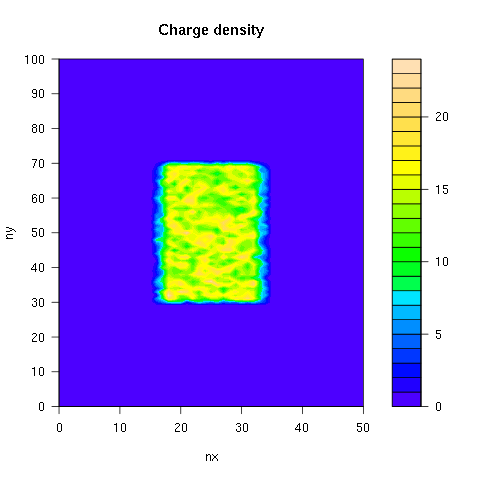
\includegraphics[scale=0.3]{./figs/out0001_density.png}
  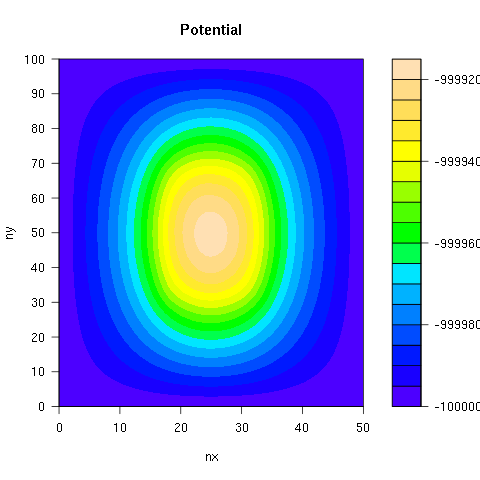
\includegraphics[scale=0.3]{./figs/out0001_potential.png}
  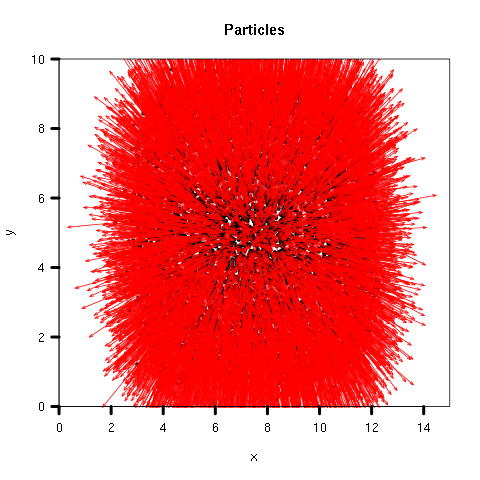
\includegraphics[scale=0.3]{./figs/out0001_particles.png}
  \caption{
    Графики плотности заряда, потенциала и распределения частиц.
  }
\end{figure}

%%% Local Variables: 
%%% mode: latex
%%% TeX-master: "major"
%%% End: 
